%!TEX root = ../../common/main.tex

\chapter{The LHCb experiment}
\label{ch:lhcb_experiment}

\section{The LHC, proton-proton interactions, and $\bquark$ hadron production}
\label{ch:lhcb_experiment:lhc}

With a circumference of \SI{26.7}{\kilo\metre} the \LHC is the largest man-made
particle accelerator. Using a \enquote{two-in-one} super-conducting magnet
design, two counter-rotating beams of protons (or ions) are intersected and
brought to collision at four interaction points, home of the large \LHC
experiments \acs*{ALICE}, \acs*{ATLAS}, \acs*{CMS}, and \acs*{LHCb}. The
colliders centre-of-mass energy of $\sqrt{s}=\SI{14}{\TeV}$ and a peak
luminosity of $L=\SI{10e34}{\lumi}$ provide \LHC's experiments with high event
rates that are necessary in their searches for physics beyond the \SM.

Following approval in 1994, the \LHC re-used the existing \LEP tunnel and most
of its infrastructure after \LEP shut down in 2000. The \LHC---and former
\LEP---tunnel is built up of eight straight and eight arc sections and has a
internal diameter of $\SI{3.7}{\metre}$. It is located north-west of Geneva,
Switzerland at a depth between $\SI{45}{\metre}$ and $\SI{170}{\metre}$ below
the surface. The storage ring consists of superconducting NbTi magnets kept at
an operating temperature of $\SI{1.9}{\kelvin}$ by superfluid helium. A
superconducting \RF cavity system captures, accelerates, and stores the two
proton beams.

At design luminosity $\num{2808}$ bunches with a bunch spacing of
$\SI{25}{\nano\metre}$ are stored in each proton beam. The \LHC relies on a
supply chain of smaller accelerators providing the initial proton bunches.

\begin{figure}[t]
  %% trim={<left> <lower> <right> <upper>}
  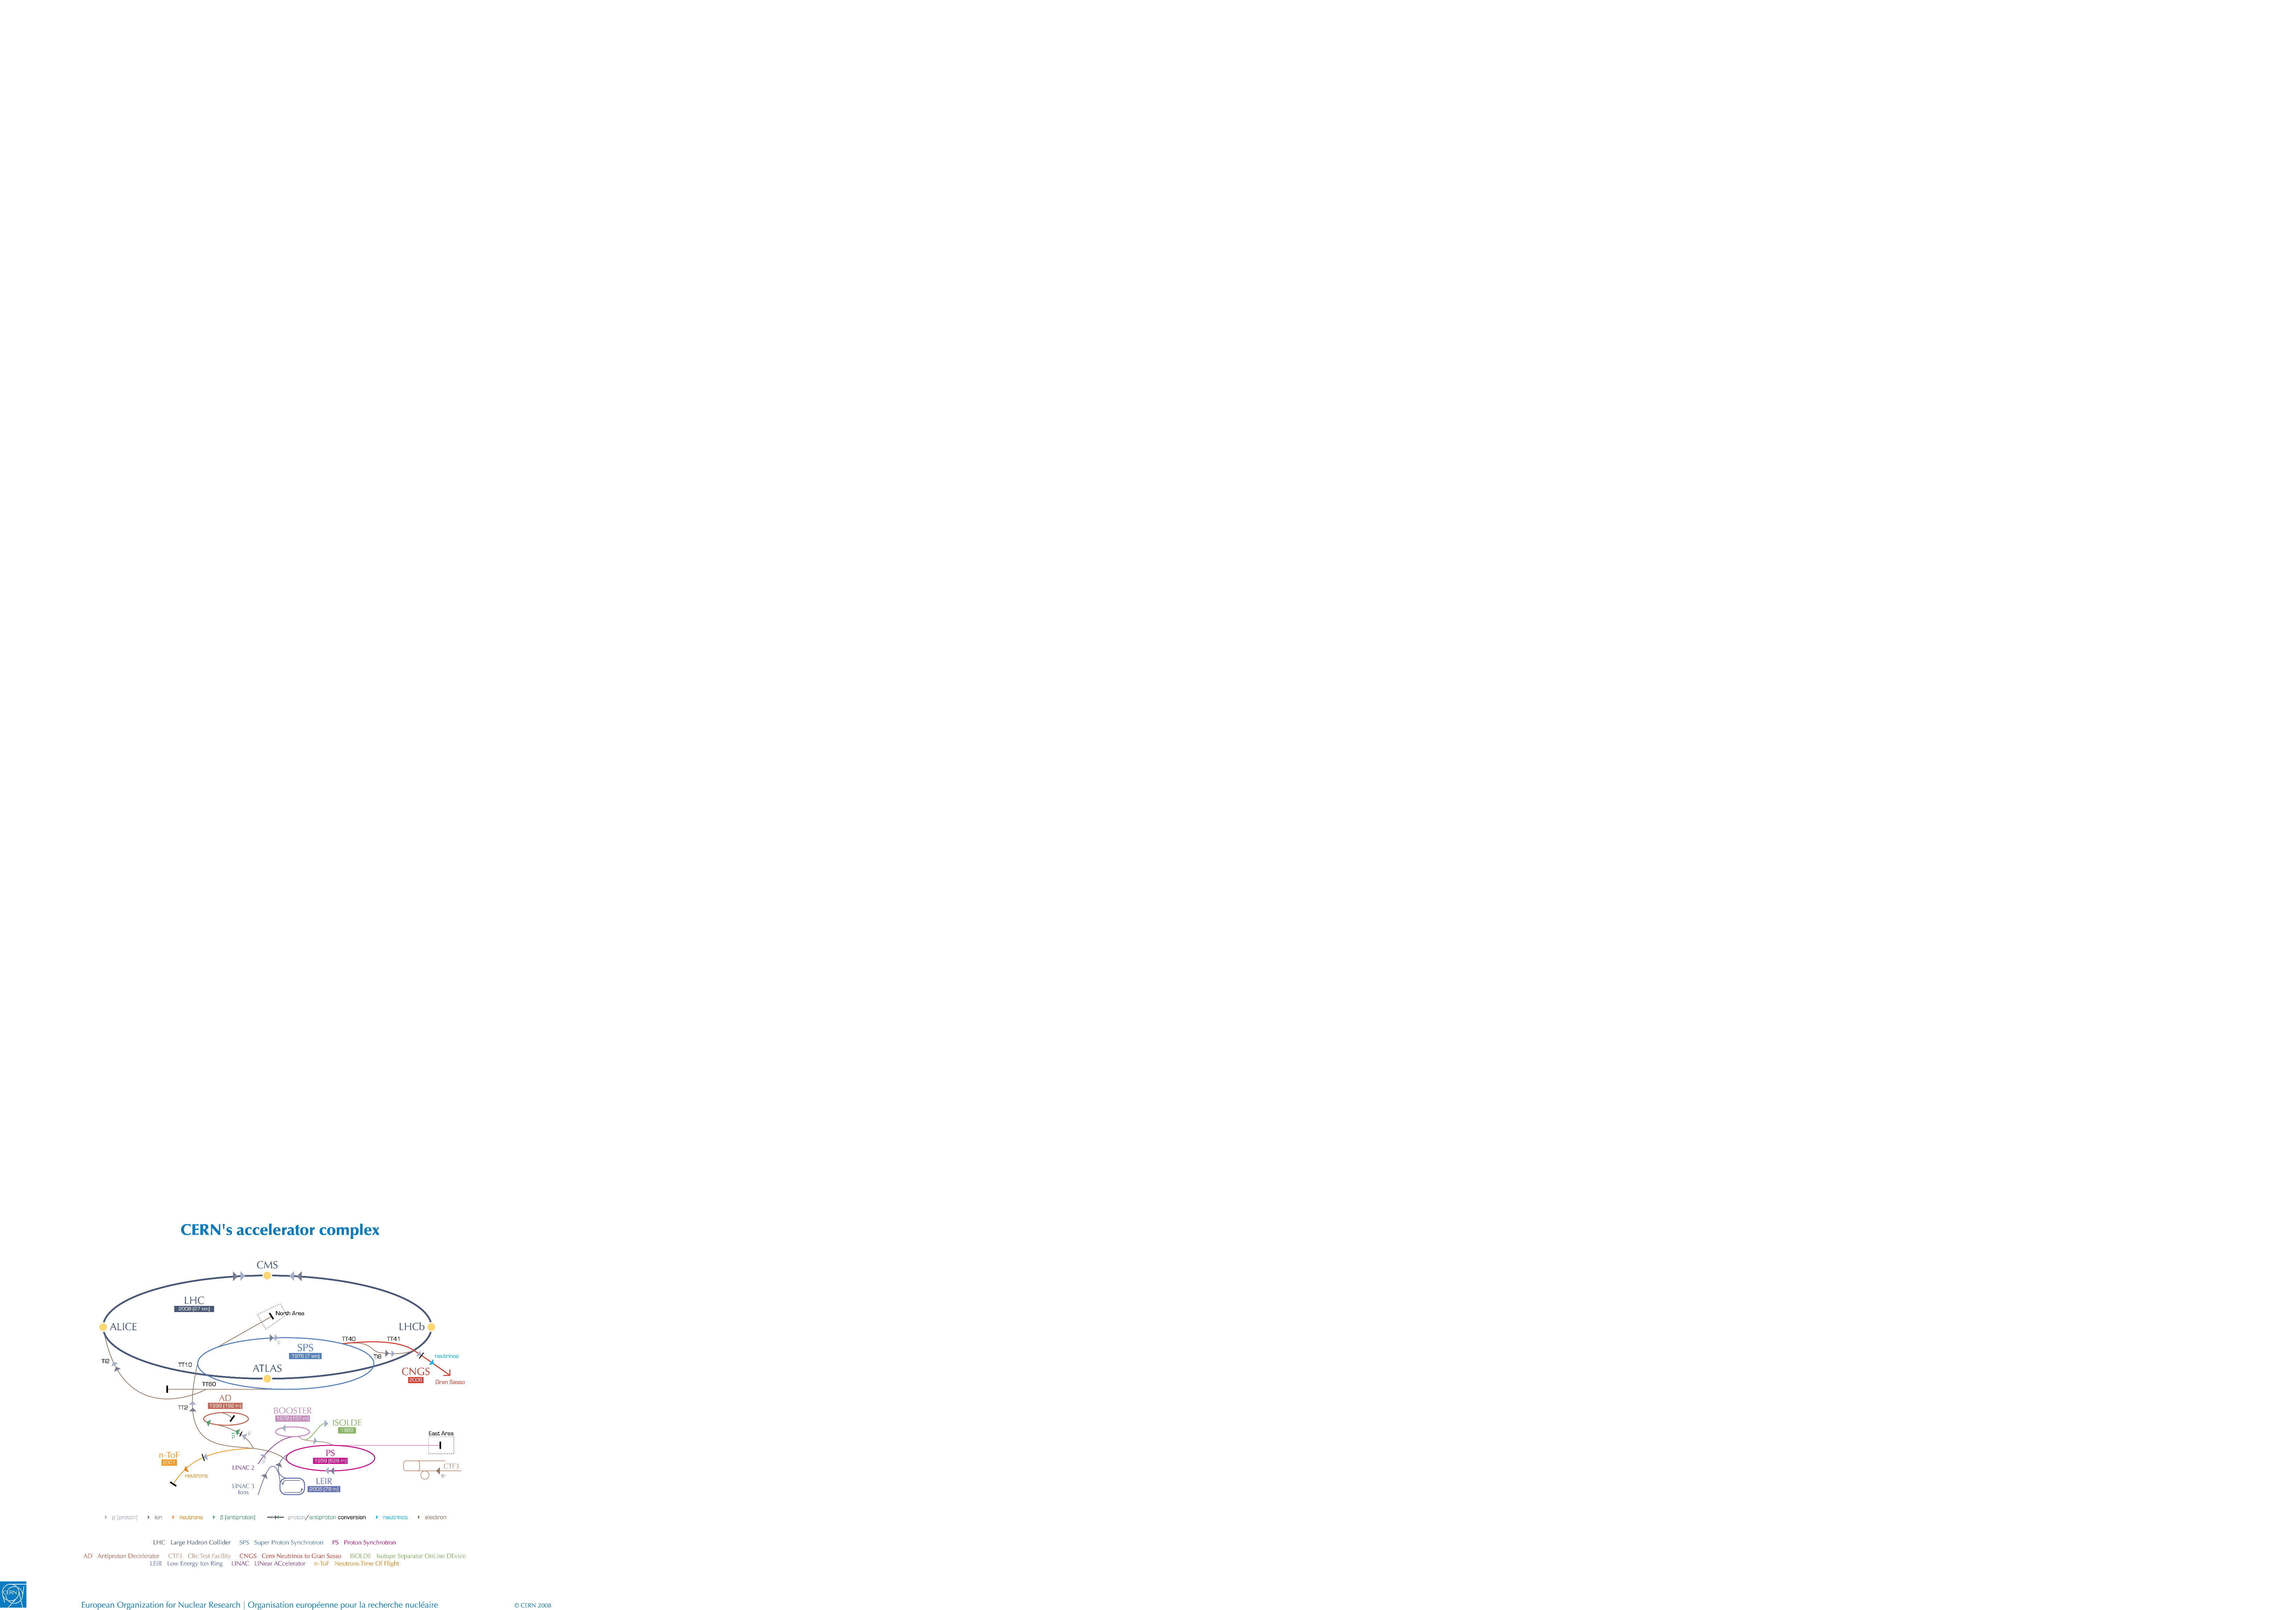
\includegraphics[width=\textwidth, trim={4.8cm 5.3cm 4.2cm 1.8cm}, clip=true]{private/content/the-lhcb-experiment/figs/cern_acceleator_complex.pdf}
  \caption{The CERN accelerator complex. \cite{Christiane:1260465}}
  \label{fig:lhcb_experiment:lhc:cern_accelerator_complex}
\end{figure}


characteristics
bunch numbers, bunch spacing, avg LHC turnaround time: total min injection time 16min, ramping from 450GeV to 7TeV approx 20min ==> minimum 70min/avg 7h, luminosity lifetime approx 15h, maximum integrated luminosity per year between 80 and 120 fb-1

experiments:
ALICE (special lumi, lead ions), ATLAS, CMS, LHCb (special lumi), TOTEM, MoDAL, LHCf

b production:
bbbar cross section, incoherent production, boost along zaxis


\section{The LHCb detector}
lumi leveling, angular acceptance, number of B decays in acceptance, production of bbar pairs
\section{Track reconstruction}
\subsection{VeLo}
\begin{itemize}
  \item purpose: displaced secondary vertices, decay length, decay time, IP
  \item silicon modules in r and phi, geometrical dimensions, mechanical accuracy, closest approach to beam
  \item acceptance: 1.6 < eta < 4.9; |z| < 10.6cm
  \item requirement of at least three hits in the VELO stations
  \item pile-up veto system
  \item retractable, RF foil, in vacuum (primary and secondary)
  \item hardware interlock system
  \item performance(?)
\end{itemize}
\subsection{TT \& IT}
\begin{itemize}
  \item silicon microstrip sensors
  \item position, geometrical dimensions, active area, x-u-v-x alignment
  \item TT pros: spatial resolution, hit occupancy, signal shaping time, single-hit efficiency, radiation damage, material budget, number of readout channels
  \item IT parts: ...
\end{itemize}
\subsection{OT}
\begin{itemize}
  \item drift-time detector, tracking of charged particles
  \item array of gas-tight straw-tube modules, each module two layers of drift-tubes
  \item drift-time < 50ns, drift-coordinate resolution 200mum
  \item three stations, each of four layers in x-u-v-x alignment, gas admixture, acceptance
\end{itemize}
\subsection{Muon}
\begin{itemize}
  \item five stations of multi-wire proportional chambers
  \item muon ID important for charmonium final states and rare decays
  \item high pT trigger for L0, and muon ID for HLT
\end{itemize}
\subsection{Track reconstruction technique and performance}
Results are form Bd2JpsiKS!
\begin{itemize}
  \item hits from VELO, TT, IT and OT are combined to form trajectories form the VELO to the calorimeters. 
  \item list different track types: long, upstream, downstream, VELO, T
  \item track seeds, Kalman filter, pattern recognition, ghosts
  \item definition of: reconstructible, successfully reconstructed
  \item performance numbers for long tracks and downstream tracks
\end{itemize}

\section{Particle identification}
\subsection{RICH}
\begin{itemize}
  \item general: cherenkov light detectors, spherical and flat mirrors, hybrid photon detectors
  \item RICH1: low momentum charged particles, 1-60GeV/c, aerogel and C4F10 radiators
  \item RICH2: CF4 gas radiator, 15-100GeV/c, reduced polar angle acceptance
  \item HPDs: 
\end{itemize}
\subsection{Calo}
\begin{itemize}
  \item trigger tasks: transverse energy hadron/electron/photon candidates for L0
  \item PID for electrons, photons, hadrons
  \item energy and position measurement
  \item design: ECAL (+SPD and PS), HCAL
  \item technical details: create scintillation light, then transmit to a photo-multiplier using fibres
\end{itemize}
\subsection{Particle identification technique and performance}
\begin{itemize}
  \item combine info from RICHs, calo, and muon system to identify: e,mu,pi,K,p also gamma, pi0
  \item hadron PID: likelihood approach, RICH pattern mached to all possible tracks under assumption of partice hypotheses. -> global pattern-recongnition
  \item RICH efficiency
  \item muon PID: extrapolating reconstructed tracks into the muon stations; considered a muon cand if a minimum number of stations have hits in their field of interest FOI
  \item muon PID efficiency
  \item lectron PID: balance of track momentum and energy of the charged cluster in the ECAL matched with extrapolated tracks; matching bremsstrahlung photons to electron tracks before the magnet
  \item gamma PID: ECAL cluster w/o associated track
  \item pi0 PID: 
  \item global performance: PV resolution of 10mum transverse to the beam and 60mum along the beam axis; invariant mass resolution between 12 and 25 MeV; lifetime resolution of around 40fs
\end{itemize}

\section{Trigger}
two level trigger system: L0 and HLT, L0 from custom made electronics, real-time with bunch crossing-frequency, HLT on software in processor farm
\subsection{L0 trigger}
from 40MHz to 1MHz, trigger on large transverse momentum pT and energy ET; the hightest ET hadron, electron, photon clusters in the calo; the two highest pT muons in the muon chambers; pile-up system in velo calculates the number of PVs; the caos calculate the total observed energy and estimate the number of tracks based on the number of hits in the SPD; using these global event cuts to reject events which would otherwise be triggered due to large combinatorics
\subsection{High level trigger}
reduced the 1MHz L0 output rate to 5kHz; software based and flexible, again composed of two parts: HLT1 and HLT2; 
\section{Online system}
\DAQ, \TFC, and \ECS
\begin{itemize}
  \item \DAQ: transport of bunch-crossing data from the detector fond-end electornics to permanent storage
  \item Front-end detector electronics -> TELL1 board : receiver cards -> \acp{FPGA} (processing, zero-suppresion, data compression) -> SyncLink (another \FPGA) collect and send raw IP-packet by GbEthernet mezzanine cards -> DAQ
  \item TELL1 has a credit-card size PC connected that interfaces to the \ECS
  \item Clock and synchronisation signals (\eg triggers) are transmitted trough the on-board \TTC interface
\end{itemize}

\section{Software stack}
\begin{itemize}
  \item \Gaudi: LHCb software framework (used by ATLAS as well)
  \item \Brunel: reconstruction
  \item \Brunel: trigger
  \item \DaVinci: end-user analysis software
  \item Simulation: \Gauss, \Boole, \Pythia, \EvtGen, \Photos, \Herwigpp, \Sherpa, \GeantFour
\end{itemize}
\section{Computing grid}
...